%%%%%%%%%%%%%%%%%%%%%%%%%%%%%%%%%%%%%%%%%%%%%%%%%%%%%%%%%%%%%%%%%%%%%%
% How to use writeLaTeX: 
%
% You edit the source code here on the left, and the preview on the
% right shows you the result within a few seconds.
%
% Bookmark this page and share the URL with your co-authors. They can
% edit at the same time!
%
% You can upload figures, bibliographies, custom classes and
% styles using the files menu.
%
%%%%%%%%%%%%%%%%%%%%%%%%%%%%%%%%%%%%%%%%%%%%%%%%%%%%%%%%%%%%%%%%%%%%%%

\documentclass[12pt]{article}

\usepackage{sbc-template}
\usepackage{amsmath,amssymb,amsfonts}
\usepackage{algorithmic}
\usepackage{textcomp}
\usepackage{xcolor}
\usepackage{hyperref}
\usepackage{graphicx,url}
\usepackage{float}

\usepackage[brazil]{babel}   
\usepackage[utf8]{inputenc}  

     
\sloppy

\title{Uma Proposta de Camada de Aplicação baseada no Padrão IEEE 11073 para Simulação de Aplicações de Saúde Digital em Redes Corporais sem Fio}

\author{Robson A. Lima, Vinicius C. Ferreira, Egberto Caballero,\\ Célio V. N. Albuquerque, Débora C. Muchaluat Saade}

\address{Laboratório MídiaCom, Instituto de Computação -- Universidade Federal Fluminense
  (UFF)\\
  Niterói -- RJ -- Brasil
  \email{\{robsonal, vinicius, egbertocr,  debora, celio\} @midiacom.uff.br}
}

\begin{document} 

\maketitle

\begin{abstract}
Simulating new protocols in WirelessBody Area Networks (WBANs) is important to evaluate new proposals before developing a real implementation. However, WBAN simulators only provide generic network applications, thus it is not possible to simulate a health device in a WBAN network. Therefore, this work proposes an application layer based on the ISO/IEEE 11073 Standard (X73-PHD) for simulating e-health applications in WBANs. Our proposal is implemented for the Castalia simulator, using the Antidote library, an open implementation of X73-PHD. Simulation results show that the X73-PHD standard communication model does not perform well due to long timeouts defined in the standard. Therefore, this paper also proposes a new communication mode, which reduces the exchange of control packets and the number of associations made by personal health devices in WBANs.
%Simulating new protocols for e-health systems is very important, as it allows an initial evaluation before a real implementation is made. On the other hand, network simulators do not offer proper support to represent medical applications or components to facilitate running simulations modeling e-health applications. Aiming at fulfilling this gap, this paper proposes a free and open-source implementation of Personal Health Devices (PHD) for Castalia Simulator. We implemented five different PHDs to act like real ISO/IEEE 11073 devices in Wireless Body Area Network (WBAN) simulations. Our implementation also supports a confirmed communication mode, where the receiver sends an  acknowledgement to the sender every time it receives a packet. Simulation results showed that the confirmed communication mode did not perform well in WBANs due to the long period of timeout proposed in the ISO/IEEE 11073 standard. Therefore, we propose an extension to the standard that decreases the overhead of control packets over the network.
\end{abstract}
     
\begin{resumo}
%Avanços na comunicação wireless e em dispositivos para saúde, tornou possível a utilização de sensores em Wireless Body Area Networks (WBANs). 
Simular novos protocolos em Redes Corporais sem Fio (Wireless Body Area Networks - WBANs) é importante para fazer uma avaliação da proposta antes de partir para desenvolver uma implementação real. Contudo, simuladores de WBANs apenas oferecem aplicações genéricas de rede, não sendo possível simular um dispositivo de saúde em uma rede WBAN. Sendo assim, este trabalho propõe uma camada de aplicação baseada no Padrão ISO/IEEE 11073 para simulação de aplicações de saúde digital em WBANs. A proposta é implementada no simulador Castalia, usando como base a biblioteca Antidote, uma implementação de código aberto de dispositivos ISO/IEEE 11073 (X73-PHD).
%Esta implementação suporta o modo de comunicação com confirmação como definido na norma, onde o receptor envia uma confirmação ao remetente toda vez que recebe um pacote. 
Resultados de simulação mostram que o modelo de comunicação padrão da norma X73-PHD não apresenta um bom desempenho devido a longos \textit{timeouts} definidos na norma. Portanto, este artigo também propõe um novo modo de comunicação, que reduz a troca de pacotes de controles e o número de associações feitas pelos dispositivos de saúde em WBANs.
\end{resumo}


\section{Introdução}\label{introduction}

%Wireless Sensor Networks (WSNs) can be applied to different scenarios, such as Internet of Things, Smart Cities, Medical Systems, etc. Due to increasing research efforts in WSN and telemedicine areas, a new type of network emerged: Wireless Body Area Networks (WBANs) or Body Area Networks (BANs) \cite{b21}. A WBAN consists of intelligent devices, attached to the skin or implanted in the body, capable of exchanging data over a wireless network \cite{b18}.
Redes de Sensores Sem Fio (RSSF) têm se tornado um ramo de estudo importante para inúmeros cenários de aplicação e simulação (internet das coisas, cidades inteligentes, informática médica, etc). Devido ao aumento de pesquisas na área de RSSF, juntamente com telemedicina, um novo tipo de rede surgiu: as redes corporais sem fio ou \textit{Wireless Body Area Networks} (WBANs) \cite{b21}. Uma WBAN é formada por dispositivos inteligentes colocados sobre pele ou implantados no corpo, que são capazes de trocar dados através de uma rede sem fio \cite{b18}. 

%The lack of commercial devices and health hazards make real experiments with WBANs rare. Therefore, simulation is an important tool to allow feasible tests with less cost and time. Castalia \cite{b15} is a widely used free and open source simulator for wireless sensor networks and wireless body area networks.
A ausência de dispositivos pessoais de saúde no mercado e os riscos que testes práticos podem oferecer à saúde tornam experimentos reais com WBANs complexos. Com o avanço e aperfeiçoamento de RSSF, simuladores se tornaram uma importante ferramenta que permite viabilizar testes com menor custo e tempo. O Castalia \cite{b15} é um simulador de redes de sensores sem fio, sensores corporais e dispositivos embutidos de baixa potência. Ele é um software livre e de código aberto, desenvolvido para que os usuários testem seus próprios algoritmos e protocolos.

%In Castalia, a body sensor is represented by a node that performs network functions, but the applications available in the simulator are generic, and do not specify the type sensor with its communication requirements.
O Castalia fornece uma estrutura genérica, confiável e realista para a primeira validação de um algoritmo, antes de passar para uma plataforma de sensor específica. Cada sensor é representado por um nó genérico, que executa funções de transmissão e recepção de dados. Entretanto, as aplicações disponíveis para testes de novos protocolos no simulador são genéricas, isto é, não especificam o tipo de sensor nem seus requisitos e procedimentos de comunicação na camada de aplicação. Isso representa um ponto fraco para o uso do simulador para aplicações de saúde digital, já que os protocolos de aplicação padronizados não são considerados nas simulações.

%In order to represent a more realistic simulation scenario, the use of a real standardized medical application is vital. The ISO/IEEE 11073 standard for Personal Health Devices (X73-PHD) describes data exchange, data representation, and terminology for communication between Personal Health Devices (PHD). Thus, this standard can be used as a role model for medical applications in our scenario.
Para tornar as simulações mais realistas, o uso de aplicações reais e padronizadas é um ponto vital. O padrão ISO/IEEE 11073 \textit{Personal Health Devices} (X73-PHD) descreve aplicações e informações para dispositivos de telessaúde. O padrão também especifica a troca e a representação de dados para comunicação entre dispositivos pessoais de saúde. Sendo assim, este artigo propõe o uso do padrão ISO/IEEE 11073 para simulação de aplicações de saúde digital em cenários de WBAN. Desta forma, simulações de novos protocolos em WBANs se tornam mais realistas com o uso de uma camada de aplicação baseada no padrão ISO/IEEE 11073.

%The term PHD involves both medical devices and health/fitness devices used in private homes \cite{b3}. The ISO/IEEE 11073 family of standards is divided into three groups, the first and oldest part is the ISO/IEEE 11073 \textit{Lower Layer}, which specifies protocols and communication service using physical layers such as infrared, wireless RF or Ethernet \cite{b16}. The ISO/IEEE 11073 \textit{Point-of-Care-Devices} (X73-PoC) specifies communication standards for devices that are used exclusively in health facilities. Finally, the X73-PHD, sets standards for personal devices used in private homes.
%VINICIUS - O que são "lay" users?, R: eu quis dizer usuários leigos mas já retirei essa palavra%
O termo PHD envolve tanto dispositivos médicos quanto dispositivos para exercícios físicos usados pelos próprios usuários em suas casas \cite{b3}. A família de normas ISO/IEEE 11073 é divida em três grupos, a primeira e mais antiga parte é a ISO/IEEE 11073 \textit{Lower Layer}, que especifica protocolos e serviços de comunicação orientados à conexão, utilizando camadas físicas como infravermelho, tecnologia RF sem fio ou Ethernet \cite{b16}. Já a parte ISO/IEEE 11073 \textit{Point-of-Care-Devices} especifica normas de comunicação para dispositivos que são usados exclusivamente em unidades de saúde. Por fim, a ISO/IEEE 11073 \textit{Personal Health Devices} (PHD), ou Dispositivo Pessoal de Saúde (DPS), define normas para dispositivos usados pelos usuários em suas casas. O foco deste trabalho será apenas na norma ISO/IEEE 11073 \textit{Personal Health Devices}, que especifica dispositivos usados mais frequentemente por usuários comuns, tais como pacientes em suas casas ou atletas que precisam ter sua atividade física monitorada, representando uma parte significativa das aplicações de saúde digital. Por questões de simplificação, esta norma será referenciada apenas como X73-PHD neste texto.

%The X73-PHD standard defines two types of devices: Agents and Managers. Agents are typically low power sensors or actuators, with limited processing power, whereas managers are devices with a greater processing power, that could be connected to an energy source.
A norma X73-PHD define dois tipos de dispositivos: \emph{agentes} e \emph{gerentes}. Os agentes são tipicamente sensores ou atuadores, de baixa potência e com pouco poder de processamento, enquanto os gerentes são dispositivos com um poder de processamento maior, que podem ou não estar conectados a uma fonte de energia. Apesar da norma X73-PHD não comentar explicitamente, dispositivos agentes e gerentes poderiam ser nós de uma WBAN.
%The goal of this work is to propose the use of ISO/IEEE 11073 standard in e-health network simulations, representing realistic medical applications and investigating the behavior of medical devices (sensors or actuators) in WBAN scenarios. Examples of personal health devices are oximeters, thermometers, ECGs, glucose meters, blood pressure monitors, etc.
%O objetivo deste trabalho, portanto, é propor uma sub-camada de aplicações médicas para o simulador Castalia, que simulará o dispositivo médico (sensor ou atuador) e analisar o comportamento desses dispositivos em redes WBAN. Alguns exemplos de dispositivos agentes simulados em redes WBAN são, termômetro, monitor de pressão sanguı́nea, medidor de glicose e etc. Todas as extensões serão desenvolvidas de acordo com a padronização de comunicação de dispositivos pessoais de saúde definidos pela norma X73-PHD.
%This paper proposes a free and open-source implementation of Personal Health Devices (PHD)  for  Castalia  Simulator.  We  implemented  five  different PHDs   to   act   like   real   ISO/IEEE   11073   devices   in   WBAN  simulations using the Antidote Library \cite{b20} as a basis.  Our  implementation also supports   a   confirmed   communication   mode,   where the receiver  sends  an  acknowledgement  to  the  sender  every  time it receives  a  packet. The 11073 standard was created as an application layer relying on reliable transport layer services. However, in many WSNs and WBAN scenarios, the transport layer is absent. Therefore, the protocol's reliable data transfer mechanism had to be adjusted to the dynamics of a faulty wireless channel, and the lack of transport layer services. Thus, we  propose  an  extension  to  the  standard  that  decreases  the overhead  of  control  packets  over  the  network.
Existem dois modos de comunicação na norma X73-PHD, o modo com confirmação e sem confirmação. No modo sem confirmação, as leituras são transmitidas sem nenhum tipo de confirmação de recebimento por parte do gerente. O modo com confirmação espera que, para cada pacote de leitura enviado pelos agentes, um \textit{acknowledgement} (ACK) seja transmitido, reconhecendo que o pacote foi entregue no gerente. De acordo com o padrão, caso o agente não receba o ACK num período de 3s, uma nova associação com o gerente deve ser feita para finalizar a transmissão de leituras. 

Este último modo de comunicação pode aumentar consideravelmente o número de pacotes de controle trocados entre agente e gerente em um cenário WBAN, quando um ACK é perdido. Para evitar esse \textit{overhead}, este artigo também propõe um novo modo de comunicação, chamado \textit{modo de retransmissão}. Este modo é baseado em \textit{stop-and-wait}, que retransmite o pacote perdido, ao invés de solicitar imediatamente uma nova associação. 

%The rest of the paper is organized as follows: In Section \ref{relatedworks}, we present related works, focusing on X73-PHD works. In Section \ref{systemarch}, an overview of our proposal is given. In Section \ref{castaliaapplayer}, we discuss the parameters available for the user to configure his/her simulation. Results are given in Section \ref{results} and, finally, conclusions in Section \ref{conclusion}.
O restante do artigo está estruturado da seguinte forma. Na Seção \ref{relatedworks}, apresentam-se trabalhos relacionados sobre o padrão X73-PHD. 
%Já na Seção \ref{systemarch}, mostramos uma visão geral do simulador e da adaptação feita na biblioteca Antidote. 
A Seção \ref{castaliaapplayer} apresenta a proposta deste artigo, detalhando o novo modo de comunicação proposto como uma extensão ao padrão X73-PHD. 
Resultados de simulações com o Castalia são discutidos na Seção \ref{results}. Por fim, as considerações finais e trabalhos futuros são comentados na Seção \ref{conclusion}.

\section{Trabalhos Relacionados}\label{relatedworks}

%The Optimized Exchange Protocol (IEEE 11073-20601) is the core of X73-PHD family. It defines the communication syntax in the Domain Information Model (DIM), machine states and services types in the Service Model and procedures in the Communication Model.
A parte IEEE 11073-20601 Optimized Exchange Protocol é o principal componente da família X73-PHD. Ele define a sintaxe de comunicação usando um Modelo de Domínio de Informação (Domain Information Model DIM), máquinas de estados e tipos de serviços de comunicação no Modelo de Serviço e procedimentos no Modelo de Comunicação

%The Domain Information Model (DIM) defines all common classes and data types used by device types. These classes are expanded by the specialization profiles according to the needs of each device. The Service Model defines the types of messages that can be exchanged between an agent and a manager and the conceptual context in which they are being transmitted \cite{b17}. The communication model defines the procedures to be followed under a normal operation, an exit condition, or when an error occurs.
O DIM define todas as classes e tipos de dados usados pelos dispositivos. Estas classes podem ser expandidas pelos agentes de acordo com a necessidade de cada um. O Modelo de Serviço define os tipos de mensagens que podem ser trocadas entre um agente e um gerente e o contexto na qual essas mensagens estão sendo transmitidas \cite{b17}. Por fim, o Modelo de Comunicação define os procedimentos a serem seguidos sob condições normais ou quando um erro ocorre.

%The 11073 family of standards includes specialization profiles, that is, each agent has an associated standard that describes its data representation. For example, the standard 11073-10408 sets standards for a thermometer, and the 11073-10415 for a balance. These specialization defines the DIM of each device, its attributes, methods, and events of each agent class.
A família de normas 11073 oferece perfis de especialização, isto é, cada agente possui suas próprias normas, as quais descrevem sua representação de dados, atributos, métodos e eventos. Por exemplo, o perfil IEEE 11073-10408 define as classes e objetos para um termômetro, já o perfil IEEE 11073-10415 faz o mesmo para uma balança. 

%Antidote Stack or Antidote Library is an implementation of the Optimized Exchange Protocol (IEEE 11073-20601) developed by Signove as part of the SigHealth Platform \footnote{SigHealth is a platform for remote patient monitoring and data management using personal wireless devices for health.}. This library is the first open source implementation of this standard, and was developed in ANSI-C with modular architecture, which allows code portability for different platforms.
A biblioteca Antidote é uma implementação da parte IEEE 11073-20601 \textit{Optimized Exchange Protocol}, desenvolvida pela empresa Signove, como parte da plataforma SigHealth\footnote{SigHealth é uma plataforma de monitoramento remoto de pacientes e gestão de dados utilizando dispositivos pessoais sem fio para a saúde.}. Esta biblioteca é a primeira implementação livre e de código aberto deste padrão, e foi desenvolvida em ANSI-C com arquitetura modular, o qual permite portabilidade de código para diferentes plataformas.

%With the popularization of the 11073 standard, several improvements were proposed to enhance the operation and interoperability. %In \cite{b7},\cite{b8} and \cite{b9} the integration of X73-PHD and IoT protocols, such as MQTT and COaP, are proposed to be used as transport protocols, enabling personal health devices to share health information directly through the Internet, using low power consumption and few control messages. Those works also discuss the availability of enabling IoT technologies for health information as well as the mapping of messages from X73-PHD into IoT protocols. All those works used real devices with Antidote as their application layer protocol.
Com o popularização da família de normas 11073, vários aperfeiçoamentos e integrações com outros sistemas foram feitos. Nos trabalhos \cite{b7}, \cite{b8} e \cite{b9}, é proposta a integração da norma X73-PHD com protocolos de IoT, como MQTT e CoAP, para serem usados na camada de transporte de PHDs. Esses protocolos auxiliariam o compartilhamento de informação de saúde diretamente na Internet, usando baixo consumo energético e poucos pacotes de controle. Nesse trabalho, também é apresentado o mapeamento das mensagens X73-PHD para mensagens MQTT e CoAP e a biblioteca Antidote é utilizada na camada de aplicação.   

%Another project on 11073 standards is \cite{b11}, which has developed an interoperable end-to-end remote patient monitoring platform using ZigBee Health Care Profile as transport layer and a Machine to Machine (M2M) solution to provide wide area network connectivity. That work also includes a web application on the clinical side (server side) and use the standards and frameworks provided by Integrating the Healthcare Enterprise (IHE) \cite{b13} and Health Level Seven (HL7) \cite{b12} to ensure end-to-end interoperability. Those two companies advocate a world in which everyone can securely access and use the right health data when and where they need it.
A norma X73-PHD é aplicada em várias áreas da saúde e de e-Health, como por exemplo, diagnóstico precoce de doenças crônicas e  monitoramento remoto de pacientes em suas residências. No trabalho \cite{b22}, os autores propõem uma coleção de dispositivos vestíveis X73-PHD, \textit{plug-and-play}, que coletam continuamente, dados fisiológicos e do ambiente. Neste projeto, três dispositivos são utilizado: dispositivos sensores, que coletam informações fisiológicas e do ambiente; Os \textit{Data Loggers}, que são dispositivos móveis, que armazenam temporariamente os dados dos sensores; e por fim, as \textit{Base Stations}, terminais que recebem, processam, armazenam e exibe informações recebidas do \textit{data loggers}. Como camada de transporte os autores, utilizaram o Bluetooth e, na camada de aplicação, o padrão X73-PHD.  

%The X73-PoC version provides a mechanism to remotely control agents. This mechanism is defined in the standards X73-10201 and X73-20301. However, the X73-PHD has no mechanisms to do such a thing. So, in \cite{b14} the author proposes to adapt the remote control capabilities from X73-PoC to X73-PHD with an acceptable overhead and no extra cost to manufacturers. This mechanism has to be installed in manager and agents, and the remote control consists of being able to change the units of measurements (e.g. - changing from kilograms to pounds) directly from the manager, a smartphone or a computer engine in nursing units.
Outro trabalho interessante é o desenvolvimento de um adaptador para dispositivos que não seguem o padrão X73-PHD. Como mostrado em \cite{b23}, os autores sugerem um dispositivo intermediário entre os sensores não padronizados e o gerente. Este dispositivo faz a tradução das mensagens vindo desses sensores para mensagens X73-PHD, e então transmite os dados traduzidos para um gerente padronizado. Este trabalho não deixa claro como foram feitos o mapeamento das mensagens e em quais dispositivos o adaptador proposto funciona. 

%In this work, we use the Antidote library to run the agent and manager X73-PHD stack over Castalia. Five different device profiles are used: 11073-10406 Basic electrocardiograph (1 to 3 lead ECG), 11073-10404 Pulse oximeter, 11073-10408 Thermometer, 11073-10417 Glucose meter, and 11073-10407 Blood pressure monitor. All these agents are used to represent body sensors in WBAN simulations. To fulfill that purpose, the X73-PHD reliable data transfer mechanism was adjusted to work on a WBAN scenario, a wireless environment, with a faulty media, and lacking transport layer services.
Neste artigo, usamos a biblioteca Antidote para propor uma camada de aplicação, seguindo o padrão X73-PHD no simulador Castalia. Cinco perfis de especialização diferentes são propostos: 11073-10406 electrocardiograma básico de 3 derivações, 11073-10404 oxímetro de pulso, 11073-10408 termômetro, 11073-10417 medidor de glicose e 11073-10407 medidor de pressão sanguínea. Além disso, um novo modo de comunicação é proposto como extensão ao padrão para uso em WBANs, como será detalhado na próxima seção.

%VINICIUS - Eu tirei pra deixar o capítulo todo mais focado em PHD%
%In \cite{b6} the authors presents an open-source energy-harvesting simulation framework called GreenCastalia which supports multi-source and multi-storage energy harvesting architectures developed for the Castalia simulator. GreenCastalia project focus is to simulate realistic battery discharge on devices. The majors modifications to the original Castalia code was made to the Resource Manager module. Also in this module the authors adds the energy-harvesting systems that provides a more realistic battery model.
%\section{Arquitetura do Sistema}\label{systemarch}

%Antidote has a plug-in based architecture. So, a Castalia plugin was developed to support communication between Antidote Stack and Castalia Modules. As the Antidote is developed to work with real devices, modifications had to be made to the library to work in Castalia Simulator. The communication, encoders, agent and manager are some of the Antidote's modules modified.
A biblioteca Antidote é portátil e usa a linguagem ANSI-C para criar um código limpo e multi-plataforma. Para realizar a comunicação entre o Antidote e outros sistemas, como o Castalia, é necessário desenvolver e adaptar plug-ins de comunicação no Antidote que permitam essa comunicação. Assim, um Plug-in para o Simulador Castalia foi desenvolvido para intermediar a comunicação com a biblioteca Antidote. Como esta biblioteca foi desenvolvida para ser usada em dispositivos médicos reais, modificações foram necessárias para que o funcionamento dentro do simulador ocorresse como em um dispositivo real. Inúmeras partes do código foram alterados, como o gerenciamento de threads, porém, os principais módulos alterados foram: \textit{communication}, \textit{encoders}, \textit{agent} and \textit{manager}.

\subsection{Castalia Plugin}

%Antidote itself is portable and uses ANSI C language to create a standard and clean library. To provide a communication between Antidote and other systems, like Castalia, we must adapt and develop the necessary communication plug-ins.
A biblioteca Antidote suporta a utilização de plug-ins para prover comunicação com o ``mundo externo''. Esses plug-ins devem ser desenvolvidos e adaptados para que se estabeleça uma comunicação entre os dois sistemas. Um dos principais desafios no desenvolvimento deste plug-in, foi adaptar o Antidote, que é escrito em C, para funcionar no Castalia, que utiliza orientação a objetos em C++. 

%The proposed plug-in allows Castalia and Antidote to talk with each other through Castalia plug-in module. Inside Castalia, we can call any function from Antidote Library and retrieve any information from it, but transmitting data from Castalia to Antidote Library is not a simple task. To solve this, we first use external variables to make the data exchange between Castalia and Castalia plug-in module. Then, to obtain the data from Castalia plug-in module, Antidote uses pointers to Castalia plug-in functions that we call \textit{callback functions}. That is why we need a plug-in to mediate the communication.
O plug-in proposto permite que o Simulador Castalia e a biblioteca Antidote conversem entre si através de um módulo que chamamos de Castalia plug-in. Dentro do Castalia podemos chamar qualquer função da biblioteca Antidote e recuperar qualquer informação dela, mas transmitir os dados do Castalia para o Antidote não é uma tarefa simples. Para resolver isso, primeiro fazemos a troca de dados entre o módulo Castalia plug-in e o Simulador Castalia. Em seguida, para obter os dados do módulo Castalia plug-in, o Antidote usa ponteiros para funções do módulo Castalia plug-in, chamadas de \textit{callback functions}. É por isso que precisamos de um plug-in para mediar a comunicação.

%There is a set of callback functions in Castalia plug-in module that are passed to Antidote during the initialization process of each agent. These callback functions are passed to communication module of Antidote as pointers to functions. This way, whenever the communication module needs to retrieve or send a message, it just triggers the correspondent callback function. The task of these callback functions is to receive and send messages as also initialize and finalize a agent network.
Há um conjunto de \textit{callback functions} que são passadas para o Antidote durante o processo de inicialização de cada agente. Essas funções são passadas para o módulo de comunicação do Antidote como ponteiros para funções. Desta forma, sempre que o módulo de comunicação precisa recuperar ou enviar alguma mensagem, ele apenas aciona a \textit{callback function} correspondente.

%Figure~\ref{fig:CastaliaPlugin} depicts how Antidote gets messages from Castalia. The arriving messages are copied to an external variable in Castalia Simulator Module - the external variable is visible to both Castalia Simulator and Castalia Plugin module. Since the communication module in Antidote owns pointers to Castalia Plug-ins functions, it can retrieve the messages using callback functions.
A Figura \ref{fig:CastaliaPlugin} descreve como o Antidote recebe as mensagens do Castalia. As mensagens que chegam são copiadas para uma variável com escopo externo no Simulador Castalia - a variável externa é visível para os módulos do Castalia e Castalia Plug-in. Como o módulo de comunicação do Antidote possui ponteiros para as funções do módulo Castalia plug-in, ele pode recuperar as mensagens usando esses ponteiros (callback functions).

%\begin{figure}[htbp]
%\centerline{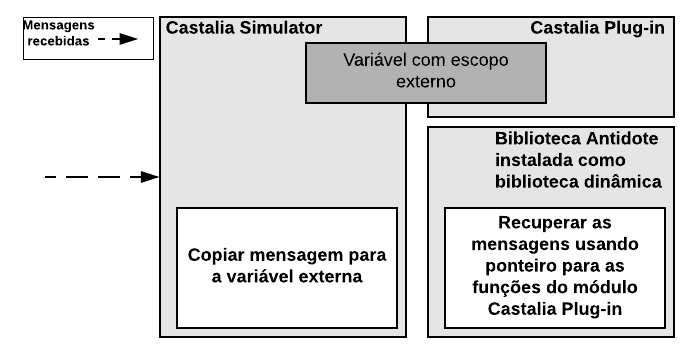
\includegraphics[scale=0.35]{figures/castaliaPlugin.png}}
%\caption{How Antidote Library gets messages from Castalia Simulator.}
%\label{fig:CastaliaPlugin}
%\end{figure}

\begin{figure}[ht]
\centering
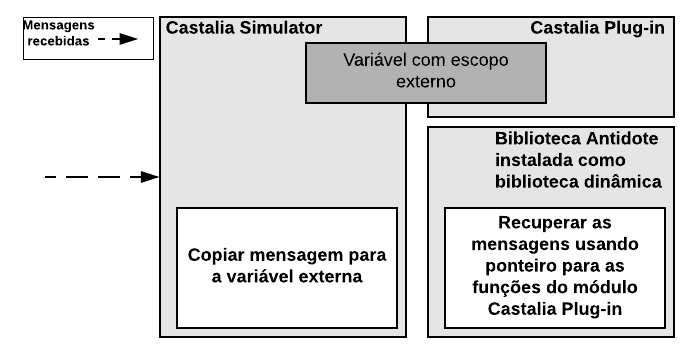
\includegraphics[width=.5\textwidth]{figures/castaliaPlugin.png}
\caption{How Antidote Library gets messages from Castalia Simulator}
\label{fig:CastaliaPlugin} 
\end{figure}

\subsection{Changes in communication module}

%The Communication module is one of the most important modules in the Antidote Library. The start, the end, transmissions, machine state phases of all nodes are controlled by this module. In a real scenario, each device has its own communication module, running its own copy of the code. But in a single-machine simulation, it is a bit different. Only one communication module has to handle all nodes, since the Antidote Library is installed in the operating system as a dynamic library.
O módulo de comunicação é um dos módulos mais importantes na biblioteca Antidote. A inicialização, a finalização, as fases da máquina de estados de todos os nós são controladas por este módulo. Em um cenário real, cada dispositivo possui seu próprio módulo de comunicação, executando sua própria cópia do código. Mas em uma simulação executada em uma única máquina é um pouco diferente. Somente um módulo de comunicação manipula todos os nós, uma vez que o Antidote é instalado no sistema operacional como uma biblioteca dinâmica.

%To ensure the proper operation of the Communication Module, the \textit{node id} is required in each function call, this way we know which node we are working with and apply the action for that node, without affecting other nodes. For example, if a node transits from unassociated state to associating machine state, without the proposed modification, this action would affect all nodes even those that should not change their machine states.
Para garantir o funcionamento adequado do módulo de comunicação, a identificação do nó é necessário em cada chamada de função, desta forma sabemos com qual nó estamos trabalhando e aplicamos a ação para apenas este nó, sem alterar o estado dos outros nós. Por exemplo, se um nó transitar do estado de máquina não associado para associando, sem a modificação proposta, essa ação afetaria todos os nós, mesmo aqueles que não deveriam alterar o estado de máquina. 

%Figure~\ref{fig:communicationModuleCastalia} illustrates the system modification. In every function in the Communication module, we insert the \textit{node id} new parameter. This way the communication module always knows the corresponding node. 
%The arrows in Fig.~\ref{fig:communicationModuleCastalia} represents functions calls.
A Figura \ref{fig:communicationModuleCastalia} ilustra a modificação do sistema. Em cada função do módulo de Comunicação, inserimos o novo parâmetro node id. Desta forma, o módulo de comunicação sempre conhece o nó em questão.

%\begin{figure}[htbp]
%\centerline{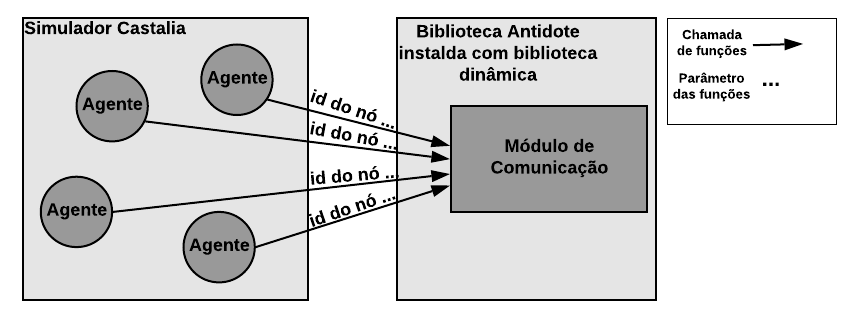
\includegraphics[scale=0.31]{figures/communicationModule.png}}
%\caption{Communication module handling several nodes. Each arrow represents a function being called from the Communication Module.}
%\label{fig:communicationModuleCastalia}
%\end{figure}

\begin{figure}[ht]
\centering
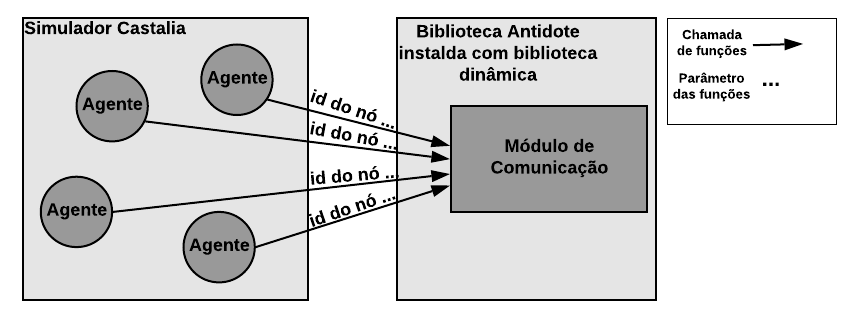
\includegraphics[width=.5\textwidth]{figures/communicationModule.png}
\caption{Communication module handling several nodes. Each arrow represents a function being called from the Communication Module}
\label{fig:communicationModuleCastalia} 
\end{figure}

\subsection{Other modifications}

%Other modules like Agent, Manager and Encoders were modified to smooth operation of Antidote functions in Castalia. We can highlight the function created in the encoder module to convert absolute values (the measurements) into scaled non-negative values as recommended by \cite{b1}. 
%Functions to finalize the Agents module were transferred to Manager module for the sake of simplicity and the \textit{node id} were add as a parameters of Agent and Manager functions. 
%In Encoder module a function to interpret the data received was created.
Outros módulos como Agent, Manager e Encoders foram modificados para facilitar o funcionamento das funções do Antidote para serem usados no Castalia. Podemos destacar a função criada no módulo do codificador para converter valores absolutos (as leituras) em valores não-negativos escalares, conforme recomendado por \cite{b1}. 

%It is useful to send absolute values like $-0.060$  which would require at least 4 bytes in X73-PHD floating point format to be sent. When converted, the number $-0.060$ becomes $388$, which requires just two bytes. The X73-PHD standard defines its own floating point types composed of a 32-bit word comprising a signed 8-bit integer exponent followed by a signed 24-bit integer mantissa.
%VINICIUS - acho melhor especificar pq falar só "many" fica muito genérico. R: feito.
Isso é útil para enviar valores absolutos como $-0.060$, o que exigiria pelo menos 4 bytes no formato de ponto flutuante da norma X73-PHD. Quando convertido, o número $-0.060$ torna-se 388, o que requer apenas dois bytes para ser enviado. O padrão X73-PHD define seus próprios tipos de ponto flutuante compostos por 32 bits que compreende um expoente inteiro com sinal de 8 bits seguido por uma mantissa de inteiro com sinal de 24 bits.

%Within the Manager, the equation to make the conversion from scaled to absolute values is given by expression\\$Y = M \times X + B$, where:
No gerente, a equação para fazer a conversão dos valores escalares para valores absolutos é dada pela expressão Y = M × X + B, onde:
\begin{align*}
    Y &= \text{valor absoluto}\\
    M &= \frac{(\text{maior valor absoluto} - \text{menor valor absoluto})}{(\text{maior valor escalar} - \text{menor valor escalar})}\\
    B &= \text{maior valor absoluto} - (M \times \text{maior valor escalar})\\
    X &= \text{valor escalar}
\end{align*}

%Within an Agent, the conversion from absolute values to scaled values is given by expression $X = \frac{(R - B)}{M}$, where: $R =$ actual measured value.
No agente, a conversão de valores absolutos para valores escalares é dada pela expressão $X = \frac{(R - B)}{M}$, onde:
\begin{align*}
   R &= \text{valor atual da leitura (valor absoluto)}
\end{align*}

%A thermometer that does readings from $-45^\circ$C  to $50^\circ$C with a resolution of $0.5^\circ$C has the following values: lower absolute value = $-45.0$, upper absolute value = $50.0$, lower scaled value = $0$, upper scaled value = $190$. Giving $M = 0.5$ and $B = -45.0$.
Um termômetro que faz leituras de $-45^\circ$C até $50^\circ$C com uma resolução de $0.5^\circ$C tem os seguintes valores:

\begin{align*}
    \text{Menor valor absoluto} &= -45.0 \\
    \text{Maior valor absoluto} &= 50.0 \\
    \text{Menor valor escalar} &= 0 \\
    \text{Maior valor escalar} &= 190
\end{align*}

%Giving $M = \frac{(50.0 - (-45.0))}{(190 – 0)} = 0.5$ and $B = 50.0 - (0.5 \times 190) = -45.0$

%The Castalia plug-in module and the modifications to Antidote Library were made exclusively for WBAN simulation in Castalia.
O módulo Castalia plug-in e as modificações na biblioteca Antidote foram feitas apenas para simulações de WBAN no Simulador Castalia. Nenhum teste foi feito em outro simulador.

%VINICIUS - talvez uma conclusão dessa seção fosse inteiressante, R: Feito
\section{Simulação de Aplicações de Saúde Digital em WBANs}\label{castaliaapplayer}

%We have created an application for the Castalia Application Layer. This application is agent-initiated, that is, the agent takes the initiative to send readings to the manager. The agent is the first and the only one to send an \textit{Association request} to start sending measurements, as well as an \textit{Association release}, when there is no more measurements to be sent.
Este trabalho propõe o uso do padrão ISO/IEEE 11073 para simulação de aplicações de saúde digital em cenários de WBAN. Conforme o padrão, são propostos um componente gerente e outro agente na Camada de Aplicação do Simulador Castalia. 
O envio de dados pode ocorrer nos dois sentidos, do gerente para o agente ou do agente para o gerente.
Entretanto, neste trabalho, o agente sempre inicia os envios de leituras para o gerente, simulando o envio de leituras de sensores ao nó concentrador da WBAN. O agente também é o primeiro e o único a enviar a mensagem de \textit{Association request} para solicitar uma associação ao gerente antes de iniciar o envio de leituras. Quando não há mais leituras para serem enviadas, o agente envia a mensagem \textit{Association release} para encerrar a associação. 

%The proposed application has five agent types, pulse oximeter, glucose meter, thermometer, blood pressure, and a basic ECG. The pulse oximeter transmits the pulse rate in beats per second and the Percentage of arterial hemoglobin oxygen saturation (SpO$_2$). The glucose meter sends the glucose level, that is, the concentration of glucose in the blood in milligrams per deciliter (mg\//dL). The thermometer measures temperature in Celsius (\textdegree C). The blood pressure sends a data compound of systolic, diastolic and the mean arterial pressure in millimeters of mercury (mmHg). The basic ECG sends eighty samples of the heart's electric potecial in millivolt (mV) per packet. Each mV sample has to be converted to scaled values before sent. 
%The lower and upper absolute values and the lower and upper scaled values are transmitted in the configuration phase. 
%All these agents samples are randomly produced, except the basic ECG that transmits real values obtained from a data base \cite{b2}.
A implementação atual oferece cinco dispositivos pessoais de saúde como agentes, um oxímetro de pulso, um medidor de glicose, um termômetro, um medidor de pressão e um eletrocardiograma (ECG de 3 derivações). O oxímetro transmite a frequência cardíaca em batimentos por minuto e a percentagem de saturação de oxigênio na hemoglobina arterial (SpO$_2$). O medidor de glicose transmite o nível de glicose, isto é, a concentração de açúcar no sangue em miligramas por decilitro (mg\//dL). O termômetro transmite a temperatura em Celsius (\textdegree C). O medidor de pressão envia uma mensagem composta por três medidas arteriais, sistólica, diastólica e a média arterial em milímetros de mercúrio (mmHg). O ECG envia oitenta amostras do potencial elétrico do coração em milivolts (mV) por pacote. 
%Cada amostra em $mV$ deve ser convertida para valores escalares antes de serem enviadas. 
%Os valores absolutos inferior e superior e os valores escalares inferior e superior são transmitidos na fase de configuração. 
Todos os dados dos agentes são produzidos de forma pseudo-aleatória, exceto o ECG que transmite valores reais obtidos a partir da base de dados \cite{b2}.

%The X73-PHD standard defines confirmed and unconfirmed events. The confirmed events expect a reception acknowledgment from the manager and the unconfirmed events do not. Control messages, like \textit{Association request} and \textit{Association release}, are always sent in confirmed mode, but measurements can be configured to use confirmed or unconfirmed mode. %The implemented parameter to set the desired mode is \textit{SN.node\[node number\].Application.confirmed\_event} which require a Boolean value.
O padrão X73-PHD define eventos com confirmação e sem confirmação. Os eventos com confirmação esperam uma mensagem de reconhecimento do gerente enquanto os eventos sem confirmação não. Mensagens de controle como \textit{Association request} e \textit{Association release} são sempre eventos que esperam uma confirmação, porém o envio de leituras pode ser ou não confirmado.

%In this application, the user can also set some simulation's parameters like: the medical device type, thermometer, pulse oximeter, blood pressure and etc, the transmission rate in measurements per seconds, the mode of operation confirmed/unconfirmed, the retransmission of the packets rather than trying a new association and the maximum number of retransmission tries.
%Na aplicação proposta para o Castalia, os usuários também definir alguns parâmetros de simulação, que são: o tipo de dispositivo a ser simulado (termômetro, oxímetro de pulso, medidor de pressão sanguínea, medidor de glicose ou ECG), a taxa de transmissão de leituras por segundo, o modo de operação, com/sem confirmação ou optar em usar nossa proposta, o modo de retransmissão.  Neste último modo o número de tentativas de retransmissão e os \textit{timeouts} podem também ser alterados.

Se um agente usa o modo de comunicação confirmado e o ACK de uma leitura enviada ao gerente não chega, o padrão indica que o agente deve realizar uma nova associação com o gerente para transmitir novamente a leitura. Em um cenário de rede sem fio, a perda de quadros pode ocorrer com frequência, por isso, o modo de comunicação confirmado proposto no padrão pode levar a uma sobrecarga de pacotes de controle com necessidade de estabelecer uma nova associação toda vez que um ACK for perdido na WBAN.

Para contornar este problema, foi utilizado o novo modo de comunicação proposto, chamado de modo de retransmissão, como extensão ao padrão ISO/IEEE 11073. As próximas subseções detalham os três modos de operação e discutem como a proposta deste artigo pode melhorar o funcionamento de \textit{Personal Health Devices} em cenários WBANs.

\subsection{Eventos sem confirmação}\label{sec:UnconfirmedMeasurementEvent}

%Figure~\ref{fig:unconfirmedMode} shows a sequence diagram of the messaging process corresponding to an ordinary operation of an agent with standard configuration and with unconfirmed measurement events. The agent intends to associate with the manager for the first time, and sends an \textit{Association request}. When the manager receives the \textit{Association request}, it checks if the manager was previously associated. If it is the agent's first association, the manager sends a \textit{Get attributes} message along with the \textit{Association response}. So, the agent sends its configuration and starts to send the measurements to the manager. When there are no more readings to transmit, the agent sends an \textit{Association release} and the manager responds with an \textit{Association release response}.
A Figura \ref{fig:unconfirmedMode} mostra um diagrama de sequência do procedimento de troca de mensagens de uma operação normal de um agente com configuração padrão e usando eventos de envio de leituras sem confirmação. O agente pretende se associar com o gerente pela primeira vez e então envia um \textit{Association request}. Quando o gerente recebe o \textit{Association request}, ele verifica se já houve associações feitas previamente com esse agente. Se for a primeira associação, o gerente envia uma mensagem de \textit{Get attributes} juntamente com uma mensagem de \textit{Association response}. Logo após, o agente envia sua configuração e atributos para iniciar a transmissão de leituras. Quando todas as leituras tiverem sido enviadas, o agente envia uma mensagem de \textit{Association release} e o gerente responde com uma mensagem \textit{Association release response} para confirmar o término desta associação.

%\begin{figure}[htbp]
%\centerline{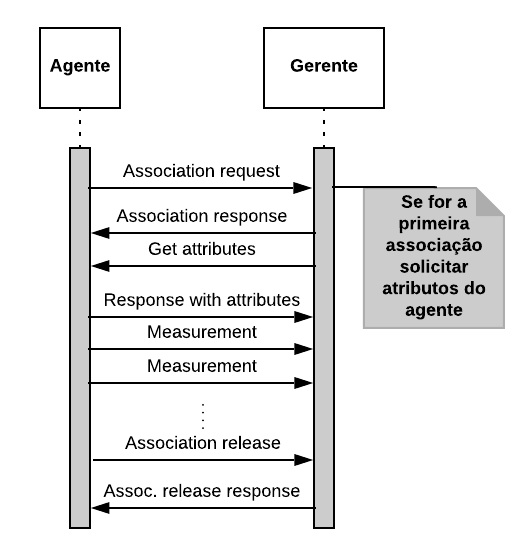
\includegraphics[scale=0.35]{figures/unconfirmed.png}}
%\caption{Sequence diagram of unconfirmed operation mode of an 11073 PHD application.}
%\label{fig:unconfirmedMode}
%\end{figure}

\begin{figure}[htbp]
\centering
\begin{minipage}{.5\textwidth}
\centering
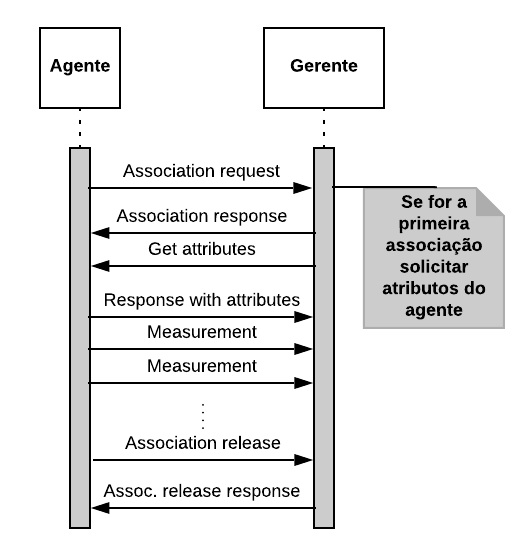
\includegraphics[width=.8\textwidth]{figures/unconfirmed.png}
\caption{Diagrama de sequência para o modo de operação sem confirmação de uma aplicação X73-PHD.}
\label{fig:unconfirmedMode}
\end{minipage}%
\begin{minipage}{.5\textwidth}
\centering
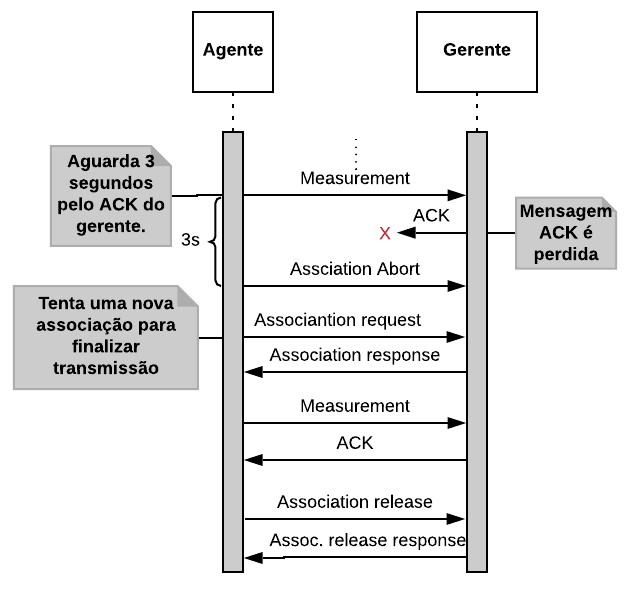
\includegraphics[width=.9\textwidth]{figures/PerdadoACKmodocomconfirmacao.png}
\caption{Diagrama de sequência para o modo de operação com confirmação de uma aplicação X73-PHD.}
\label{fig:confirmedMode} 
\end{minipage}%
\end{figure}

\subsection{Eventos com confirmação}

%\begin{figure}[htbp]
%\centerline{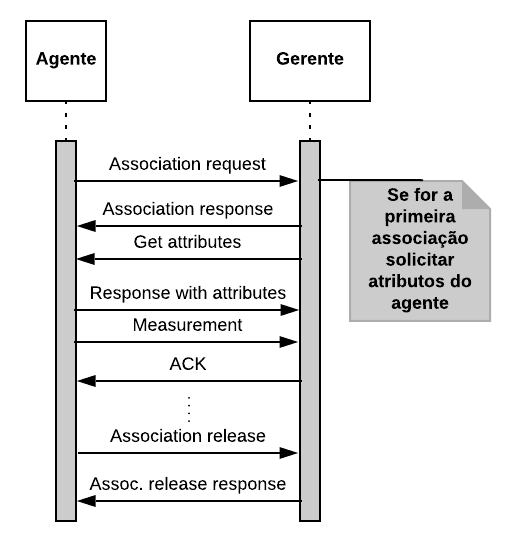
\includegraphics[scale=0.35]{figures/confirmed.png}}
%\caption{Sequence diagram of confirmed operation mode of an 11073 PHD application.}
%\label{fig:confirmedMode}
%\end{figure}

%\begin{figure}[htbp]
%\centering
%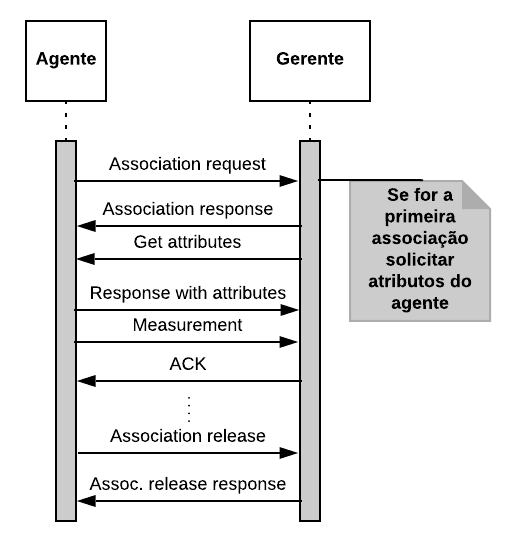
\includegraphics[width=.5\textwidth]{figures/confirmed.png}
%\caption{Diagrama de sequência para o modo de operação com confirmação de uma aplicação X73-PHD.}
%\label{fig:confirmedMode} 
%\end{figure}

%Figure~\ref{fig:confirmedMode} depicts a sequence diagram of the messaging procedure corresponding to an operation of an agent with standard configuration and with confirmed measurements events. The initial procedure is the same as explained in Section \ref{sec:UnconfirmedMeasurementEvent}, the difference is that the manager sends an acknowledgment for every measurement received. After sending a measurement data, the agent must wait three seconds for an ACK. If an ACK is not received in this period, the agent sends an \textit{Association abort} to the manager, and transits to the unassociated state. If the agent still has readings to send, a new association must be made. % VINICIUS - Reescreve isso aí, pq não deu pra entender - This and others errors conditions is explained in \cite{b1}.
A Figura \ref{fig:confirmedMode} descreve o diagrama de sequência da operação de um agente com configuração padrão usando eventos de envio de leitura com confirmação. O processo inicial é idêntico ao explicado na Seção \ref{sec:UnconfirmedMeasurementEvent}. A diferença é que para cada leitura que o agente envia, o gerente confirma com uma mensagem ACK. Após enviar uma leitura, o agente espera a confirmação por três segundos, se nada chegar durante esse período, o agente envia uma mensagem de interrupção, \textit{Association abort}, e transita para o estado de máquina não associado. Se ainda existirem leituras para serem enviadas, o agente deve tentar uma nova associação.

\subsection{Proposta de Modo de Retransmissão}

%The X73-PHD standard assumes that there will be a reliable transport layer on real devices. In the Castalia simulator, as in usual wireless sensor networks, a transport layer is not used. So we propose a stop-and-wait system as a sub-application-layer to retransmit agent packets whose ACK have not been received.
O padrão X73-PHD assume que, em dispositivos reais, haverá um camada de transporte confiável disponível para comunicação, como  o \textit{Bluetooth Health Device Profile} ou \textit{ZigBee}. Em uma WBAN, pode não haver camada de transporte confiável disponível, já que os sensores têm poucos recursos de memória, processamento e bateria. Desta forma, este artigo propõe um novo modo de comunicação, baseado em \textit{stop-and-wait}, para realizar retransmissões de pacotes perdidos ou não confirmados pelo gerente.

%To avoid many associations right after a non-received ACK we implemented a stop-and-wait retransmission system in the application layer. 
%It reduces the unnecessary exchange of several control packets made in association procedures. Rather than making a new association when an ACK is lost, we just retransmit the packet $n$ times or until an ACK is received.
%The user can define whether to retransmit and how many retransmission attempts wish.
%The user may define a number ($n$) of retransmissions, and the agent will retransmit that message up to $n$ times until a corresponding ACK is received. If the manager receives a duplicated message, it will retransmit immediately another ACK to the agent.
Isso reduz a troca desnecessária de vários pacotes de controle no processo de associação. Ao invés de fazer uma nova associação quando um ACK não é recebido, retransmite-se o pacote até que um ACK seja recebido. O usuário define o número $n$ de retransmissões, e, então, aquela leitura será retransmitida até $n$ vezes ou até que um ACK seja recebido. Se o gerente receber uma mensagem duplicada, ele retransmitirá imediatamente o ACK que não foi recebido pelo agente, ou seja, o último ACK enviado.

Na fase de associação, a implementação reduz o \textit{timeout} de $10$ para $0.4$ segundos. Após a associação, o dispositivo usando o \textit{o Modo de Retransmissão}, envia sua primeira leitura, aguarda o período de \textit{timeOutToRetransmitPacket} conforme definido pelo usuário no arquivo de configuração da simulação. Se nenhuma resposta for recebida, o pacote é retransmitido no máximo \textit{maxNumOfRetransmition} vezes, conforme definido também pelo usuário, ou até que uma mensagem de reconhecimento do gerente seja recebida. Se todas as tentativas definidas em \textit{maxNumOfRetransmition} forem utilizadas, então uma nova associação é feita com o gerente e a variável \textit{maxNumOfRetransmition} é redefinida para $0$. Esse processo continua até o agente realizar $3$ associações, conforme definido no padrão X73-PHD. Na quarta tentativa, o agente envia uma mensagem de \textit{Association abort} e volta para estado de máquina \textit{não associado}. 

%In Section \ref{results}, we evaluate this solution's efficiency in reducing control packets exchange in a WBAN scenario. Note that this is a new proposal, not present in the X73-PHD standard. 
%The parameters implemented for retransmission are \textit{SN.node[nodeNumber].Application.retransmissionPacket} which require a boolean value and \textit{SN.node[nodeNumber].Application.maxNumOfRetransmition} that accepts an integer number.
Na Seção \ref{results}, é avaliada a eficiência desta proposta usando como métrica a redução no envio de pacotes de controle, o número de novas associações feitas por cada dispositivo, a quantidade de pacotes retransmitidos e a número de leituras transmitidas com sucesso para o gerente. Vale ressaltar que esta é uma nova proposta e não está presente no padrão X73-PHD.

A implementação no simulador Castalia foi realizada utilizando a biblioteca Antidote \cite{b20} como base. Ao usar a nova camada de aplicação disponível, os usuários também podem definir alguns parâmetros de simulação, que são: o tipo de dispositivo a ser simulado (termômetro, oxímetro de pulso, medidor de pressão sanguínea, medidor de glicose ou ECG), a taxa de transmissão de leituras por segundo, o modo de operação, com/sem confirmação ou optar em usar a proposta deste artigo, o modo de retransmissão.  Neste último modo, o número de tentativas de retransmissão e os \textit{timeouts} também podem ser configurados.

\section{Resultados}\label{results}
%All results presented in this section are relative to the application layer. We run simulations on a computer with 2GB RAM memory, CPU intel dual core i3, and Ubuntu 18.04.1 LTS operating system. All runs last 101 seconds with the first second used just for network setup (e.g., nodes requesting connections). The simulation was executed 20 times with $95\%$ of confidence interval.
%Using some \textit{api} from Castalia Simulator some results like the total number of control packets exchanged, the total number of measurements packets, how many times a packets was retransmited among many others results can be obtained easily.
Todos os resultados apresentados nesta seção são relativos à camada de aplicação implementada por este trabalho. As simulações foram feitas em um computador com 8GB de mémoria RAM, Intel Core i5-7200U e sistema operacional Ubuntu 18.04.1 LTS. A simulação tem duração de $101s$, sendo o primeiro segundo apenas para a configuração da camada MAC. Foram executadas $15$ repetições da simulação com intervalo de confiança de $95\%$. 
%Devido à escala de alguns gráficos, nem sempre o intervalo de confiança fica muito visível. 

\subsection{Casos de Uso e Parâmetros da Simulação}

%Remote Monitoring and Independent living for elderly care is one of the use cases of the X73-PHD standard. The sensors and actuators proposed for this use case are: blood pressure, thermometer, glucose meter, pulse oximeter and basic ECG  \cite{b3}. In this work, we have used an hypothetical elderly patient who has cardiac problems, diabetes and hypertension, and needs to be monitored in his home.
Monitoramento remoto de pacientes e independência para a terceira idade são casos de uso discutidos na norma X73-PHD. Os sensores e atuadores propostos para esses dois casos de usos são: medidor de pressão, termômetro, medidor de glicose, oxímetro de pulso e um eletrocardiograma.

%Figure~\ref{fig:wbantopology} shows the topology setup used in our simulation. The hub node is placed at the right hip, a sensor node at each wrist, one sensor node at the each ankle, and one sensor on the chest. We used this set to test our proposed features. These nodes' positions have the advantage of experimental measurements of path loss, made for every pair of nodes, as discussed in \cite{b4}.
A Figura \ref{fig:wbantopology} mostra a topologia utilizada nas simulações. O hub, que é o nó gerente, está localizado no quadril direito, um nó sensor em cada pulso e um em cada tornozelo e um sensor no meio do peito. Utilizando essas posições, temos a vantagem de utilizar um canal sem fio que já possui um modelo de perda de sinal, entre cada par de dispositivos, pré-definido com experimentos reais, conforme apresentado em \cite{b4}.

%\begin{figure}[htbp]
%\centerline{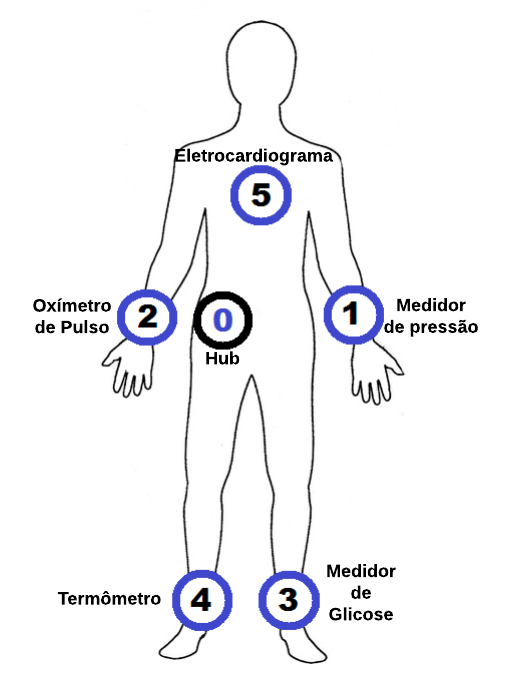
\includegraphics[scale=0.29]{figures/corpoSensoresNomes.png}}
%\caption{The simulated network topology.}
%\label{fig:wbantopology}
%\end{figure}

\begin{figure}[htbp]
\centering
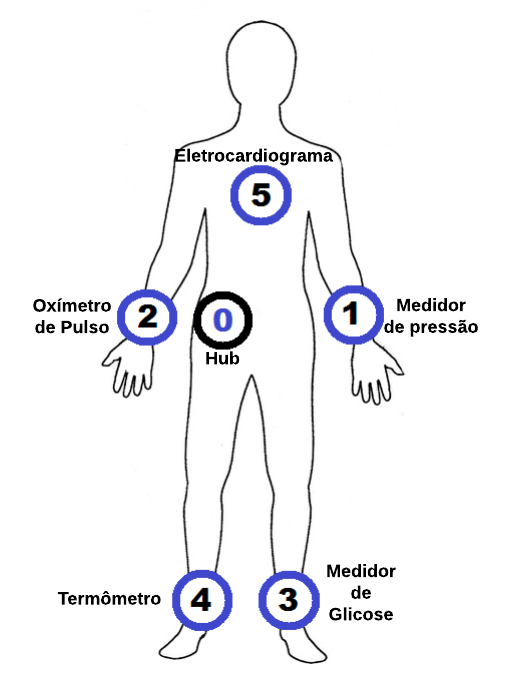
\includegraphics[width=.3\textwidth]{figures/corpoSensoresNomes.png}
\caption{Topologia da rede utilizada nas simulações.}
\label{fig:wbantopology} 
\end{figure}

%In this work, we simulate three scenarios. In the first scenario, called \textbf{unconfirmed mode}, agents send measurements with no confirmation by the manager. In the second scenario, called \textbf{retransmission mode}, agents expect an ACK from the manager during three seconds and in case it is not received, the packet is retransmitted up to three times, after that, a new association is made. The third and last one, \textbf{confirmed mode}, agents wait for three seconds the ACK from the manager. If an ACK is not received, the agent has to try to establish a new association to finalize the transmission of the measurement packets. Table \ref{3modes} summarizes the three mentioned modes.
%Neste trabalho, nós simulamos três cenários diferentes. No primeiro cenário, chamado de \textbf{unconfirmed mode}, os agentes enviam leituras sem esperar nenhuma confirmação do gerente. No segundo cenário, \textbf{retransmission mode}, onde é aplicado nossa proposta, os agentes esperam por confirmação por cada pacote de leitura enviada e, fazem a retransmissão dos pacotes caso uma confirmação não seja recebida. No terceiro e último cenário, \textbf{confirmed mode}, os agentes esperam uma confirmação durante três segundos, se um ACK não for recebido neste período, uma nova associação é estabelecida para finalizar a transmissão dos pacotes.  A tabela \ref{3modes} resumo os três cenários apresentados.
O cenário de simulação utilizado foi definido da seguinte forma: utilizando o modo de retransmissão, os agentes esperam por uma confirmação do pacotes por um tempo definido pelo usuário no parâmetro  \textit{timeOutToRetransmitPacket}, se nenhuma confirmação é recebida, é feita a retransmissão desse pacote por até \textit{maxNumOfRetransmition} vezes, também definido pelo usuário. Se o valor \textit{maxNumOfRetransmition} de retransmissões for atingido, uma nova associação é estabelecida. Foram usados cinco valores diferentes para \textit{timeOutToRetransmitPacket}, $200$, $400$, $600$, $800$ e $1000$ milissegundos. Para \textit{maxNumOfRetransmition} utilizamos $6$, $7$, $8$, $9$ e $10$, totalizando 25 cenários diferentes.

%The MAC layer used is the IEEE 802.15.6 (WBAN) \cite{b5} with path loss map and temporal model for wireless channel supplied by Castalia, and we use a 1024 Kbps physical data rate. The radio used meets with the IEEE 802.15.6 radio proposal \cite{b5} with $-15$dBm as transmission power.
%VINICIUS - Faltou colocar as referências para o padrão do MAC e dizer quantas retransmissões são usadas no retransmission mode% R: Feito
Foi utilizada a camada MAC definida pela norma IEEE 802.15.6 (WBAN) \cite{b5} com mapa de perda de sinal e modelo temporal para o canal sem fio fornecidos pelo simulador Castalia. A taxa de transmissão da camada física foi definida para $1024$ Kbps e o rádio utilizado se enquadra nas proposta do padrão IEEE 802.15.6, trabalhando com $-15$dBm para transmissão.

%\begin{table}[htbp]
%\caption{Modos de operação implementados na aplicação proposta}
%\begin{center}
%\begin{tabular}{lllll}
%\cline{2-4}
% & \multicolumn{1}{c}{\textbf{\begin{tabular}[c]{@{}c@{}}Modo\\ sem confirmação\end{tabular}}}                      & \multicolumn{1}{c}{\textbf{\begin{tabular}[c]{@{}c@{}}Modo com\\ retransmissão\end{tabular}}}                                      & \multicolumn{1}{c}{\textbf{\begin{tabular}[c]{@{}c@{}}Modo com\\ confirmação\end{tabular}}}                                         &  \\ \cline{2-4}
%& \begin{tabular}[c]{@{}l@{}}As leituras \\ são transmitidas\\ sem confirmação \\ do gerente.\end{tabular} & \begin{tabular}[c]{@{}l@{}}As leituras \\ são retransmitidas\\ se um ACK não\\ for recebido\\  do gerente.\end{tabular} & \begin{tabular}[c]{@{}l@{}}Se um ACK não\\ for recebido, tente\\ uma nova associação\\ para continuar a transmissão \\das leituras.\end{tabular} &  \\ \cline{2-4}
%\end{tabular}
%\label{3modes}
%\end{center}
%\end{table}

%The configuration of the nodes is set as follows: the total simulation time is 100 seconds. Node 0 uses the \textit{Manager} application and is the hub. The blood pressure and the pulse oximeter transmit one measurement per second, totalizing 100 measurements to be sent in our simulation. The thermometer sends one read every 2 seconds, then, 50 measurements should be sent. The glucose meter transmits one measurement every 25 seconds, that is, 4 measurements in 100 seconds. In this work, we assume the basic ECG as a device that receives signals of all electrodes deployed in the body, and transmit these signals to the manager. It will transmit 80 millivolt samples per 0.8 seconds, which gives 125 measurement packets in 100 seconds of simulation.
As configurações dos nós é definida da seguinte forma: O nó zero é o hub e usa a aplicação \textit{Manager}. Os demais nós são agentes e usam a aplicação \textit{Agent}. Ambas as aplicações foram desenvolvidas por este trabalho. O medidor de pressão e o oxímetro de pulso transmitem uma leitura por segundo para o gerente, totalizando $100$ leituras durante toda a simulação. O termômetro envia uma leitura a cada 2 segundos, assim, 50 leituras devem ser enviadas durante a simulação. O medidor de glicose transmite apenas uma leitura a cada 25 segundos, totalizando no final da simulação 4 leituras a serem enviadas. Neste trabalho, é assumido que o ECG é um dispositivo que recebe os sinais de todos os eletrodos que estiverem implantados no corpo e envia os sinais para o gerente. Este ECG transmitirá $80$ leituras por pacote a cada $0.8$ segundos, o que no final totaliza 125 leituras. Essas $80$ amostras equivalem a $0.8$ segundos de dados retirados da base de dados \cite{b2}.

\subsection{Análise dos resultados}

%All the results that will be presented is already implemented in the proposed application and everyone can feel free to customize it. 
%The results available in the application are the total control packets exchanged per node, the measurements packets received by the manager per node, the measurements packets sent by each node, and the total of associations made per agent. 

% The first result discussed is the total of successfully measurements delivered to the manager. As described in \cite{b1}, when an agent is working on confirmed mode, it  should send a measurement packet and wait for the ACK during three seconds. 
Analisar a quantidade de leituras que foram entregues com sucesso no gerente é fundamental para averiguar a eficiência do método de transmissão. Na Figura \ref{fig:leiturasEntregues}, é exibida a quantidade de leituras entregues por cada um dos dispositivos, em cada um dos vinte e cinco cenários analisados, utilizando o mecanismo proposto e, na Figura \ref{fig:leiturasEntregues2modes} é possível ver o desempenho dos três modos onde, foi utilizado o cenário \textit{maxNumOfRetransmition} = 6 e \textit{timeOutToRetransmitPacket} = 200ms para o modo de retransmissão. 

\begin{figure}[htbp]
\centering
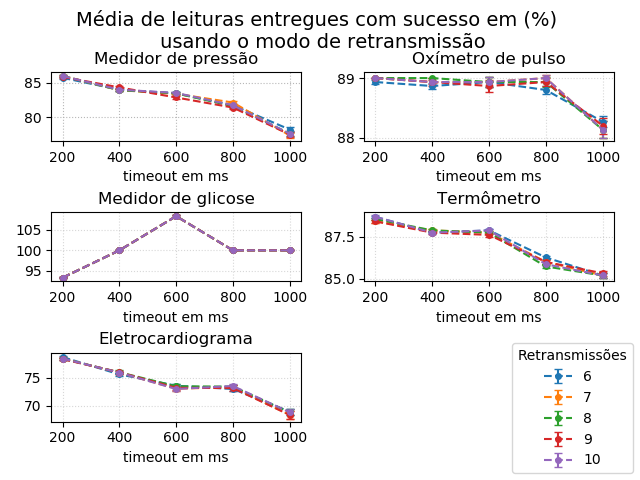
\includegraphics[width=.7\textwidth]{figures/mediaDeLeiturasEntregues.png}
\caption{O eixo $y$ representa a percentagem de leituras entregues e o eixo $x$ os valores de  \textit{timeOutToRetransmitPacket}. Cada linha do gráfico representa um valor de \textit{maxNumOfRetransmition}.}
\label{fig:leiturasEntregues} 
\end{figure}

É possível observar na Figura \ref{fig:leiturasEntregues} que a maioria dos pacotes são transmitidos quando o menor \textit{timeout} de $200$ milissegundos é utilizado. Este resultado é esperado, pois a simulação possui tempo finito e, quanto maior o \textit{timeout}, menos tempo para enviar leituras o dispositivo possui. Por outro lado, a qualidade do enlace sem fio e a quantidade de leituras transmitidas influenciam diretamente neste resultado. Enquanto o medidor de glicose envia apenas quatro leituras em $100s$, o ECG - que possui o pior link entre todos os dispositivos, tem que enviar 125 em $100s$ apenas.

\begin{figure}[H]
\centering
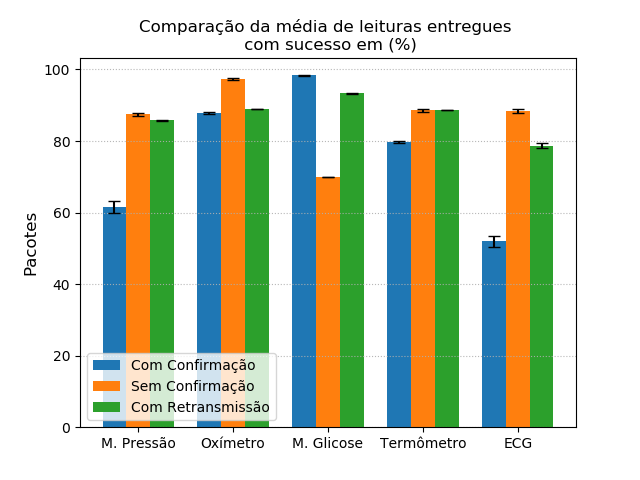
\includegraphics[width=.6\textwidth]{figures/mediaDeLeiturasEntregues2modes.png}
\caption{O eixo $y$ representa a percentagem de leituras entregues e o eixo $x$ os agentes. Cada linha do gráfico representa um modo de operação.}
\label{fig:leiturasEntregues2modes}
\end{figure}

% We can see in Fig.~\ref{fig:measurementreceivedpernode} the lack of adaption of the confirmed mode to the scenario, due to lost ACKs, timeouts and disassociation/reassociation processes. The retransmission mode improved the results by reducing the wait time of an association handshake, and retransmitting the messages sooner. The unconfirmed mode delivered almost all packets, although it provides no reliability.
%VINICIUS - Poderia quantificar a melhoria do retransmission em relação ao confirmed%

No modo de operação com confirmação, apenas o oxímetro e medidor de glicose entregaram mais de $85\%$ das leituras. Devido o modo de operação sem confirmação não utilizar nenhum mecanismo de entrega confiável e nenhum \textit{timeout} durante a transmissão, obteve um bom desempenho em quase todos os dispositivos.

% The overhead of control packets exchanged between a node and the manager is crucial in this scenario, as in the case of a new association due to a non-received ACK. The association procedure involves a maximum of four packets for a new node, and a minimum of two packets, when the agent's attributes are previously known.

% The total average of control packets exchanged between each node and the manager per operation mode is depicted in Fig.~\ref{fig:controlpacketsexchanged}. Notice that our retransmission mode saves about $21.5\%$ of control packets when compared to the confirmed mode. The unconfirmed mode as expected is the one that transmits less control packets.
Podemos observar que existe um \textit{trade-off} quando $200$ milissegundos é utilizado como \textit{timeout}. Na Figura \ref{fig:retransmicoes}, é possível ver que o maior número de retransmissões ocorreu quando $200$ milissegundos foi utilizado. Isso acontece em razão do gerente não enviar uma resposta dentro do tempo limite, fazendo com que os agentes reenviem o pacote por falta de ACK. O gráfico apresentado possui apenas valores do cenário onde \textit{maxNumOfRetransmition} é igual a $6$, pois, a partir da sétima retransmissão, os valores tendem a ficar próximos de zero, como pode ser visto na Figura \ref{fig:retransmicoes}.

\begin{figure}[htbp]
\centering
\begin{minipage}{.5\textwidth}
\centering
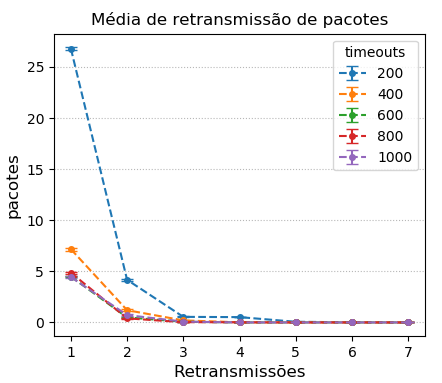
\includegraphics[width=.9\textwidth]{figures/retransmicoes.png}
\caption{Retransmissões de pacotes utilizando \textit{timeouts} diferentes.}
\label{fig:retransmicoes}
\end{minipage}%
\centering
\begin{minipage}{.5\textwidth}
\centering
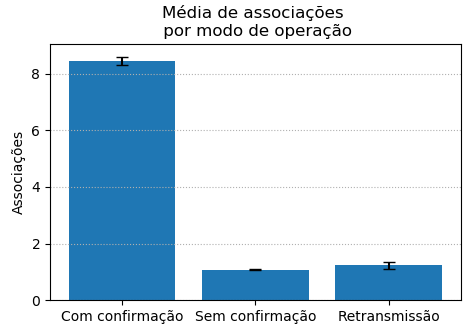
\includegraphics[width=.9\textwidth]{figures/associacoes.png}
\caption{Média de associações feitas por agente, para o cenário com \textit{maxNumOfRetransmition} = $6$ e  \textit{timeOutToRetransmitPacket} = $600$ ms.}
\label{fig:associacoes} 
\end{minipage}
\end{figure}

Pode-se ver a redução no número de associações feitas por cada agente, entre o modo de operação com confirmação e o modo proposto no artigo na Figura \ref{fig:associacoes}. Em média, no modo de retransmissão, cada agente precisou estabelecer menos de duas associações para concluir a transmissão de leituras, enquanto o modo com confirmação usou em média mais de oito associações em cada transmissão. Isso representa uma economia de até 32 pacotes de controles, e vários \textit{timeouts} evitados. 

% \begin{figure}[htbp]
% \centering

% \end{figure}

% The number of associations made per node is extremely high with the confirmed mode, since it tries a new association after every packet lost. Fig.~\ref{fig:associationnumber} shows the average number of associations that each node made in the three operation modes. As expected, the confirmed mode has the highest average of association attempts, while the unconfirmed mode made just one association. The retransmission mode tries a new association after all the attempts to resend a message fail, or if the agent receives an abort message from the manager. This is the reason for the low average of associations in this mode.   
Na Figura \ref{fig:latencia}, nota-se que a maioria dos pacotes possuem uma latência média de $30$ milissegundos. O tempo é calculado desde a criação do pacote, na camada de aplicação do agente, até o recebimento do mesmo na camada de aplicação do gerente. Os valores mostrados são referentes ao cenário onde \textit{maxNumOfRetransmition} é igual a $6$ e  \textit{timeOutToRetransmitPacket} é igual a $200$ ms.

\begin{figure}[htbp]
\centering
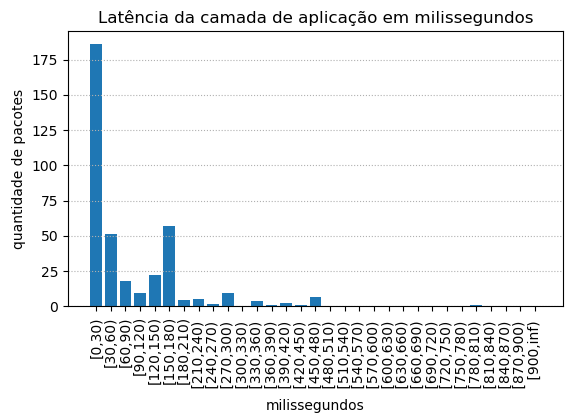
\includegraphics[width=.6\textwidth]{figures/latencia.png}
\caption{Latência média da camada de aplicação dos agentes, para o cenário com \textit{maxNumOfRetransmition} = $6$ e  \textit{timeOutToRetransmitPacket} = $200$ ms.}
\label{fig:latencia} 
\end{figure}

Como visto nos resultados apresentados, o modo sem confirmação obteve uma das melhores performances, pois não possui nenhum tipo de mecanismo de entrega confiável e nem confirmação de entrega. O modo de retransmissão, alcançou um bom desempenho mesmo perdendo às vezes para o modo sem confirmação. Este modo entregou cerca de $15\%$ mais pacotes de leituras e economizou $20.5\%$ pacotes de controle, quando comparado ao modo com confirmação. Este último, infelizmente, demanda muito tempo e associações, o que resulta num \textit{delay} alto e poucos pacotes entregues com sucesso.





\section{Conclusão}\label{conclusion}
%In this paper, we have presented a proposal to simulate personal health devices in Castalia Simulator. Our application layer follows the X73-PHD standard with the aid of the Antidote Library. Five agents were implemented, and they simulate real personal health devices. In adittion, a new reliable data transfer mode was proposed, the retransmission mode, to adjust the X73-PHD protocol to WBAN scenarios, where a reliable transport layer is usually not available. The retransmission mode aimed at reducing the number of disassociation/reassociations that take place after a message or acknowledgement is lost.
Neste artigo, foi apresentada uma extensão ao protocolo X73-PHD que pode ser testado no Simulador Castalia e, adaptou dispositivos X73-PHD para serem empregados em cenários WBAN.
Como ilustrado nos resultados, esta proposta melhora o desempenho dos PHDs, ao mesmo tempo que oferece um mecanismo de entrega confiável. 

%As future work, we intend to develop a manager-initiated transmission, where the user can set the amout of measurements each agent must collect. The codes for Castalia Application and for Antidote Modified Library can be found respectively at \url{https://github.com/conqlima/Antidote} and \url{https://github.com/conqlima/11073PhdApplication}.
Como trabalhos futuros, será desenvolvida a função que permite ao usuário especificar, no gerente, a quantidade de dados que deve ser transmitida por cada agente. Os códigos da Aplicação do Castalia e da biblioteca Antidote modificada, podem ser encontrados nos endereços: \url{https://github.com/conqlima/Antidote} e \url{https://github.com/conqlima/11073PhdApplication}. 
%The results shows the advantages of using the retransmission mode over the standards' confirmed mode, increasing the message delivery ratio and reducing the overhead of the protocol. 



%\begin{figure}[ht]
%\centering
%\includegraphics[width=.5\textwidth]{fig1.jpg}
%\caption{A typical figure}
%\label{fig:exampleFig1} 
%\end{figure}

%\begin{table}[ht]
%\centering 
%\caption{Variables to be considered on the evaluation of interaction
%techniques}
%\label{tab:exTable1}
%\includegraphics[width=.7\textwidth]{table.jpg}
%\end{table}

\bibliographystyle{sbc}
\bibliography{newbib}

\end{document}
